
\chapter{Capital Asset Pricing Model}\label{CAPM}

\section{Principios básicos}

Se conoce con el nombre de Modelo de Valuación de Activos de Capital (CAPM, por sus siglas en inglés), a la teoría desarrollada principalmente por William Sharp en 1964 en base a trabajos previos de Harry Markowitz y James Tobin \cite{sharp}. Mediante este modelo se puede determinar la relación entre la rentabilidad de un activo cualquiera y su riesgo asociado, por lo que es de gran utilidad en la teoría de administración de portafolios de inversión. 

Un portafolio perfectamente diversificado, que contenga todos los activos existentes en el mercado, no es afectado por las variaciones particulares que pueda sufrir un activo\footnote{Para una comprobación rigurosa, véase Elton y Gruber (1995).\nocite{elton}}. Esto se debe a que el riesgo individual de cada activo es muy pequeño en comparación con la cartera, por lo que lo único que es relevante en este caso es el riesgo sistémico\footnote{Riesgo sistémico es aquel que afecta a todo el mercado, como puede ser una noticia de orden macroeconómico.}. Ahora, si consideramos al mercado como base de análisis, cada activo tendrá una sensibilidad mayor o menor a las variaciones de la economía.

Lo enunciado en el párrafo anterior es una explicación conceptual del CAPM. Considerando el razonamiento de un inversor racional y averso al riesgo, para realizar una inversión que tenga riesgos asociados, siempre se esperará que el rendimiento sea mayor a la tasa pagadera por un activo libre de riesgo.

Este modelo presenta una forma de equilibrio general que permite ver la relación entre riesgo y rentabilidad de los activos \cite{elton}. La ventaja de esta relación es que hace al CAPM capaz de valuar cualquier tipo de activo en el mercado. Se considera un mundo ideal con el objetivo de agregar simplicidad al modelo, lo que implica tomar en cuenta una serie de supuestos \cite{elton}.

Primero, se asume la ausencia de costos de transacción, ya que de otra forma habría que considerar el hecho de si el inversor ya poseía activos en su cartera, o los adquirió posteriormente. 

Segundo, los activos se consideran infinitamente divisibles, esto es esencial ya que un portafolio bien diversificado (como uno equivalente a todo el mercado) debe contener una parte pequeña de cada activo. 

En tercer lugar se asume la inexistencia de efectos fiscales como el impuesto a las ganancias, de esta forma se eliminan todas las distorsiones que estos puedan provocar. 

Cuarto, un solo inversor no puede afectar el precio de un activo, ya que esto provocaría variaciones en los precios de los activos por el solo hecho de adquirirlos, lo que desvirtuaría el análisis completamente. 

El quinto supuesto esta relacionado con la forma en la que los inversores toman sus decisiones. Debido a que el CAPM utiliza como base un portafolio equivalente al mercado, es necesario que este sea eficiente y que los otros agentes de mercado armen su cartera racionalmente maximizando el rendimiento para un nivel de riesgo.

En sexto lugar, los inversores pueden realizar de manera ilimitada ventas en corto (\textit{short sales}), así como pueden colocar y pedir prestado a la tasa de interés libre de riesgo.

Por último, se considera que todos los agentes de mercado disponen de la misma información y por lo tanto hay homogeneidad de expectativas. A su vez, es necesario remarcar que los activos deben ser comerciables, aspecto que no necesariamente se cumple en mercados no desarrollados por razones de iliquidez.


\section{El problema del inversor}

\subsection{La utilidad obtenida}

Tomando el supuesto de que una persona cualquiera toma sus decisiones de inversión en base a la rentabilidad y el riesgo esperado \cite{sharp}, es posible analizar como será su selección de activos.

Existen dos formas funcionales esenciales para analizar la selección de activos. Primero, la función de utilidad de un inversor que puede expresarse en términos de rentabilidad esperada \cite{sharp}:

\begin{align}
	U = U(\overline{r_i} ; \sigma_i) \label{funcionutilidad}
\end{align}

Donde $\overline{r_i}$ es la rentabilidad esperada de la inversión y $\sigma_i$ es el riesgo, medido como el desvío entre la rentabilidad esperada y la posiblemente obtenida. $U$ en función del rendimiento será positivo ($\partial U/\partial r_i > 0$) debido a que un inversor obtendrá lógicamente mayor utilidad a medida que la rendimiento aumenta, manteniendo el riesgo constante. Inversamente, $U$ en función del riesgo será negativo ($\partial U/\partial \sigma_i < 0$), \textit{ceteris paribus}.

\begin{figure}[H]
\centering
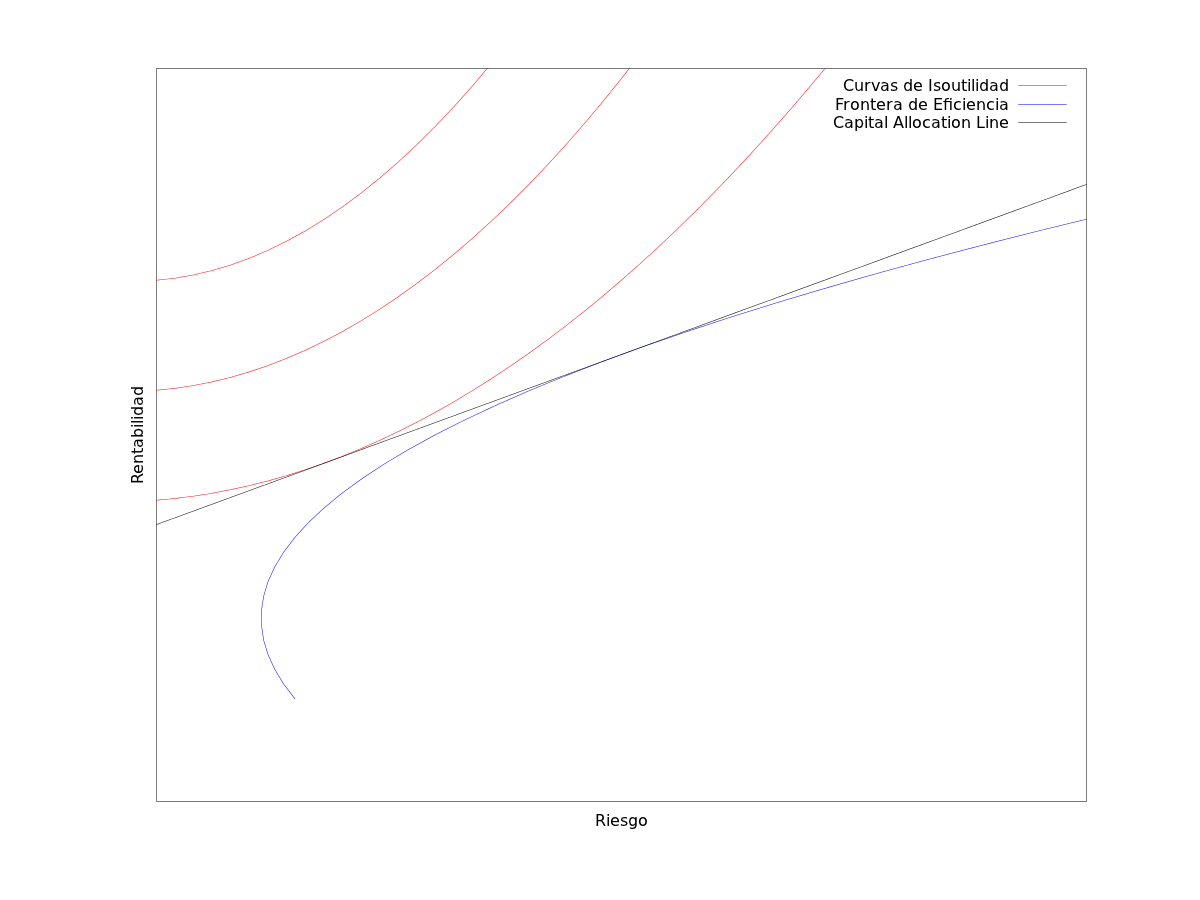
\includegraphics[width=1\textwidth]{Images/capm.png}
\caption{Frontera de eficiencia, \textit{CAL} y curvas de isoutilidad}
\label{fig:frontef}
\end{figure}

La figura \ref{fig:frontef} muestra las curvas de isoutilidad, es decir que todos los punto sobre cada una de ellas representan la misma utilidad para el inversor. La elección entre dos portafolios ubicados sobre la misma curva de isoutilidad le es indistinta al inversor. Cuanto más arriba se encuentre la curva, mayor utilidad total presentará debido a que de dos portafolios con el mismo riesgo siempre es preferible aquel que se espera tenga mayor rendimiento. De la misma forma, de dos portafolios con el mismo rendimiento esperado, siempre es preferible el que tenga menor riesgo.

Resolver el problema del inversor consistirá en encontrar el portafolio que maximice la utilidad del inversor, sujeto a la limitación de los posibles portafolios construibles.

\subsection{Selección de portafolio}

La segunda función a analizar es la de la frontera de portafolios posibles. Si un inversor decide distribuir el total de su capital en dos o más activos de riesgo, de acuerdo a como distribuya su capital, podrá obtener distintos portafolios resultantes. En el caso en que dichos activos no se encuentren perfectamente correlacionados, la función resultante de opciones posibles será una curva convexa que se encuentre por sobre todos los activos considerados. Esta curva, o frontera de eficiencia, se encuentra representada en la figura \ref{fig:frontef}.

La forma de la frontera de eficiencia se debe a que la correlación no es perfecta entre todos los activos \cite[p.430]{sharp}. Esto es demostrable fácilmente si se calcula el desvío esperado de una combinación de dos activos riesgosos, ya que la tanto el rendimiento como el desvío dependerán de las proporciones invertidas en cada activo, este último de forma no lineal. Por ejemplo, si se deposita $\alpha$ en el activo 1 y $(1-\alpha)$ en el activo 2, el retorno y el desvío del portafolio resultante serán: 

\begin{align}
	\overline{r_P} &= \alpha \overline{r_1} + (1-\alpha) \overline{r_2} \label{renddosactivos} \\
	\sigma_P &= \left[ \alpha^2 \sigma_1^2 + (1-\alpha)^2 \sigma_2^2 + 
		2 \alpha (1-\alpha) \sigma_{12} \right]^{1/2} \label{desviodosactivos}
\end{align}

Donde $\overline{r_P}$ y $\sigma_P$ son el rendimiento esperado y el desvío de los rendimientos del portafolio, $\overline{r_i}$ y $\sigma_i$ son el rendimiento esperado y el desvío de los rendimientos del activo $i$, y $\alpha$ es la proporción invertida en el activo 1.

Una vez construida la frontera de eficiencia, producto de la combinación de activos riesgosos, se debe seleccionar el portafolio adecuado. Si se toma como supuesto que el inversor puede colocar y tomar prestado a la tasa libre de riesgo ($r_f$), el portafolio final resultante ($P$) será entonces una combinación lineal entre esta y el portafolio riesgoso ($Z$). Por ende, $P$ será el resultado de la combinación entre $Z$ y $r_f$, siendo este último un activo sin riesgo y por ende no correlacionado con $Z$.

Las diferentes combinaciones entre $Z$ y $r_f$ crean el conjunto de portafolios posibles. Cuando todos los portafolios combinación de estos se encuentran  sobre todo el conjunto abarcado por la frontera de eficiencia, entonces la recta que surge de unir estos dos puntos maximiza la elección del inversor.. A esta recta se la conoce como \textit{Capital Allocation Line} (\textit{CAL}) y se encuentra representada en la figura \ref{fig:frontef}. La \textit{CAL} es entonces la recta de mayor pendiente, que maximiza a su vez la utilidad del inversor.

Extendiendo las ecuaciones \eqref{renddosactivos} y \eqref{desviodosactivos} al caso de $n$ activos, el rendimiento esperado del portafolio se calculará como el promedio ponderado de los activos que lo componen. En el caso del riesgo del portafolio, o desvío estándar de los rendimientos, este se calcula como muestra la ecuación \eqref{varportafolio}.

\begin{align}
	\overline{r_P} &= w_1 \overline{r_1} + w_2 \overline{r_2} + \dotsb + 
		w_n \overline{r_n} = \sum\limits_{i=1}^n w_i \overline{r_i} \label{rendportafolio} \\
	\sigma_P^2 &= \sum\limits_{i=1}^n w_i^2 \overline{r_i}^2 + 
		\sum\limits_{i=1}^n \sum\limits_{\substack{j=1 \\ i \neq j}}^n w_i w_j \sigma_{ij}  \label{varportafolio}
\end{align}

Donde $w_i$ es la proporción del activo $i$ en la cartera. A continuación se deriva la fórmula de la pendiente de la \textit{CAL} para el caso de $n$ activos.


\section{Portafolio óptimo}

Como puede apreciarse en la figura \ref{fig:frontef}, la pendiente de la \textit{CAL} ($\theta$) puede ser expresada de la siguiente forma:

\begin{align}
	\theta = \frac{\overline{r_P} - r_f}{\sigma_P}
\end{align} 

Para obtener el conjunto de portafolios eficientes es necesario encontrar la recta que posea mayor pendiente. Esto se debe a que al maximizarla, sea cuales sean las curvas de isoutilidad del inversor, la máxima utilidad se obtendrá en la intersección con la \textit{CAL}.

Entonces, maximizando la pendiente:

\begin{align}
	\mbox{max } \theta = \frac{\overline{r_P} - r_f}{\sigma_P} \label{maxptecal}
\end{align}

Con respecto a $w_i$ y sujeto a:

\begin{align}
\mbox{Restricciones} \left\{  \nonumber
	\begin{array}{l}
		\mbox{1) } \overline{r_P} = w_1 \overline{r_1} + w_2 \overline{r_2} + \dotsb + 
			w_n \overline{r_n} = \sum\limits_{i=1}^n w_i \overline{r_i} \nonumber\\
		\mbox{2) } \sigma_P^2 = \sum\limits_{i=1}^n w_i^2 \overline{r_i}^2 + 
			\sum\limits_{i=1}^n \sum\limits_{\substack{j=1 \\ i \neq j}}^n w_i w_j \sigma_{ij}  \nonumber \\
		\mbox{3) } \sum\limits_{i=1}^n w_i = 1
	\end{array} \right.
\end{align}

La primer y tercer restricción pueden ser reemplazadas en la fórmula de la pendiente de la CAL. Debido a que $\sum w_i r_f = r_f$, se obtiene que $\theta$ estará dado por:

\begin{align}
	\theta = \left[ \sum\limits_{i=1}^n w_i (\overline{r_i} - r_f) \right] 
		\left( \sum\limits_{i=1}^n w_i^2 \overline{r_i}^2 + \sum\limits_{i=1}^n 
		\sum\limits_{\substack{j=1 \\ i \neq j}}^n w_i w_j \sigma_{ij} \right)^{-1/2}
\end{align}

Ahora, derivando $\theta$ en función de cada proporción en la cartera $w_i$ e igualando a cero, es posible obtener el máximo de la función. Esto quiere decir que el resultado que maximice la pendiente de la CAL será aquel que haga cero todas las derivadas parciales de la misma. Formalmente:

\begin{align}
	\frac{\partial \theta}{\partial w_i} = 0 \quad \forall \quad 1 \leq i \leq n
\end{align}

Entonces, igualando la derivada a cero y despejando se llega a lo siguiente:

\begin{align}
	\overline{r_i} - r_f = \frac{\sum\limits_{i=1}^n w_i (\overline{r_i} - r_f)}{\sigma^2} 
		\left( w_i \sigma_i^2 + \sum\limits_{\substack{j=1 \\ j \neq i}}^n w_j \sigma_{ij} \right) \label{eqzetas1}
\end{align}

El primer término de la ecuación \eqref{eqzetas1} es igual a la rentabilidad en exceso del portafolio divido su desvío: $ (\overline{r_P} - r_f)/\sigma_P^2$. Para simplificar se puede llamar $Z_i$ a esto último multiplicado por la proporción de cada activo en el portafolio ($w_i$):

\begin{align}
	Z_i = \frac{\overline{r_P} - r_f}{\sigma_P^2} * w_i \label{formulazeta}
\end{align}

De esta forma obtenemos un conjunto de ecuaciones, una por cada derivada parcial de la ecuación \eqref{maxptecal} o, lo que es lo mismo, una por cada activo en el portafolio del inversor.

\begin{align}
	\left\{
	\begin{array}{l l}
		\overline{r_1} - r_f &= Z_1 \sigma_1^2 + Z_2 \sigma_{1 2} + \dotsb + Z_n \sigma_{1 n} \\
		\overline{r_2} - r_f &= Z_1 \sigma_{2 1} + Z_2 \sigma_2^2 + \dotsb + Z_n \sigma_{2 n} \\
		& \mbox{ }\vdots \\
		\overline{r_n} - r_f &= Z_1 \sigma_{n 1} + Z_2 \sigma_{n 2} + \dotsb + Z_n \sigma_n^2 
	\end{array} \right. \label{eczetas}
\end{align}


El sistema de ecuaciones \eqref{eczetas} resuelve la combinación óptima de activos según la teoría desarrollada por Markowitz. Este sistema puede ser fácilmente resuelto usando un sistema de matrices para averiguar los valores de $Z_i$. Luego, las proporciones pueden ser obtenidas haciendo $w_1 = \frac{Z_1}{\sum Z_i}$, $w_2 = \frac{Z_2}{\sum Z_i}$, ..., $w_n = \frac{Z_n}{\sum Z_i}$.

Con este método un inversor racional armaría su portafolio, lo que nos permite llevar este modelo aún más lejos y analizar el caso en donde todos los inversores optimizarían su portafolio de la misma forma. Esto si bien es hipotético dada la naturaleza de la afirmación, puede ser tomado como un supuesto válido para el modelo presentado a continuación.

\section{Derivación del CAPM}

Como se mencionó anteriormente, la teoría desarrollada por Harry Markowitz es la base de este modelo. Dicha teoría postula una forma eficiente de combinar activos cuando se forma una cartera de inversión, de forma de maximizar el rendimiento esperado dado un nivel de riesgo.

Si en el mercado existen una gran cantidad de activos riesgosos, la combinación de estos en diferentes cantidades pueden producir una infinita variedad de resultados. Sin embargo, en caso de existir dos activos con el mismo nivel de riesgo y diferente rentabilidad, un inversor racional sólo compraría el que tenga mayor rentabilidad. Más aún, lo lógico sería vender el activo que se espera que tenga un rendimiento menor  y con el dinero obtenido comprar de mayor ganancia esperada. Dado que en los dos activos el riesgo es igual, la ganancia en promedio será positiva. Esta clase de operaciones tendería a incrementar el precio de las acciones con mayor rendimiento esperado y a reducir el precio del resto. La dinámica generada por la oferta y la demanda de activos, crea una situación de equilibrio en donde todos los activos con igual riesgo poseen igual rendimiento esperado \cite{sharp}.

El inversor analizado en la sección anterior puede decidir diversificar su portafolio en una gran cantidad de activos, idealmente infinitos, para diluir el riesgo particular de cada activo \cite{effectofdiversification}. Si las proporciones de su portafolio se vuelven iguales a las proporciones de los activos en el mercado, se puede decir que su portafolio es igual al del mercado (en términos de $w_i$). Para el caso bajo análisis la fórmula \eqref{formulazeta} queda:

\begin{align}
	Z_i = \frac{\overline{r_M} - r_f}{\sigma_M^2} * w_i \label{formulazetamercado}
\end{align}

Nótese que la única diferencia entre \eqref{formulazeta} y \eqref{formulazetamercado} es que la segunda considera el rendimiento esperado del mercado (notado $\overline{r_M}$) y la varianza del mismo, las cuales son iguales a las del portafolio. Ahora, tomando un activo cualquiera, la ecuación del portafolio óptimo \eqref{eqzetas1} queda:

\begin{align}
	\overline{r_i} - r_f = \frac{\overline{r_M} - r_f}{\sigma_M^2} 
		\underbrace{\left( \sum\limits_{j=1}^n w_j \sigma_{ij} \right)}_{Cov(r_i; r_M)}
\end{align}

Debido a que el segundo término es igual a la covarianza entre los rendimientos de $i$ y los del mercado
\footnote{Demostración: \begin{align}
		Cov(r_i, r_M) &= E[(r_i-\overline{r_i})(r_M-\overline{r_M})] \nonumber\\
			&= E[(r_i-\overline{r_i})(\sum\limits_{j=1}^n w_j r_j-\sum\limits_{j=1}^n w_j \overline{r_j})] \nonumber\\
			&= \sum\limits_{j=1}^n w_j E[(r_i-\overline{r_i})(r_j-\overline{r_j})]
			= \sum\limits_{j=1}^n w_i \sigma_{ij} \nonumber
		\end{align}}, se puede despejar la rentabilidad del activo:

\begin{align}
	\overline{r_i} = r_f + \frac{Cov(r_i; r_M)}{\sigma_M^2} ( \overline{r_M} - r_f )
\end{align}

Finalmente, la expresión $ Cov(r_i; r_M) / \sigma_M^2$ puede ser reemplazada con la letra griega $\beta$. \textit{CAPM} se expresa normalmente de la siguiente forma:

\begin{align}
	\overline{r_i} = r_f + \beta ( \overline{r_M} - r_f ) \label{capm}
\end{align}

La letra \textit{beta} representa la relacion de rentabilidad y riesgo histórico entre un activo y un portafolio igual al mercado. El hecho de que sea una relación histórica se debe a que normalmente el \textit{beta} se obtiene mediante una regresión lineal de los valores del mercado. Esto no niega que el \textit{CAPM} sea adecuado al mostrar la relación entre rentabilidad y riesgo, al menos en el largo plazo \cite[p.357]{elton}.


\section{Características de \textit{Beta}}

Como se explicó en la sección anterior, el \textit{beta} de un activo es igual a la covarianza del mismo contra el mercado, dividido la varianza del mercado. Si la varianza del mercado en un momento particular está dada, dos activos con distinta covarianza con el mercado tendrán diferente \textit{beta}. A mayor covarianza la $\beta$ será también mayor. 

Que un activo posea $\beta = 1$ significa que un cambio en el mercado provocará un cambio de igual magnitud en dicho activo, o al menos eso se espera. La razón de esto es que la \textit{beta} del mercado es por definición igual a uno, al ser la covarianza entre dos rendimientos iguales (mercado contra mercado) igual a la varianza ($\sigma_M^2 / \sigma_M^2 = 1$). Si el \textit{beta} es mayor que uno, un movimiento sistémico producirá un cambio aún mayor en el activo. Lo opuesto ocurrirá si $\beta < 1$.

Cuando un portafolio se encuentra altamente diversificado, los \textit{shocks} particulares de cada activo tienen a ser insignificantes y desaparecer en el portafolio \cite{sharp}. Es por esto que el impacto que sufre un activo en particular debido a \textit{shocks} sistémicos es el único relevante, siendo esto lo que el \textit{beta} mide.

El \textit{beta} de un portafolio puede ser calculado a partir del rendimiento esperado para un conjunto de $n$ activos, utilizando \textit{CAPM}:

\begin{align}
	\sum\limits_{i=1}^n w_i \overline{r_i} &= \sum\limits_{i=1}^n w_i \left[ r_f + 
		\beta_i (\overline{r_M} - \overline{r_f}) \right] \label{sumatoriacapm} \\
	\mbox{con } \sum\limits_{i=1}^n w_i &= 1 \nonumber
\end{align}

Como $\sum w_i \overline{r_i} = \overline{r_P}$, reorganizando la ecuación \eqref{sumatoriacapm} obtenemos:


\begin{align}
	\underbrace{\sum\limits_{i=1}^n w_i \overline{r_i}}_{r_P} &= r_f + 
		\underbrace{\sum\limits_{i=1}^n \beta_i}_{\beta_P} (\overline{r_M} - \overline{r_f}) \label{betaportafolio}
\end{align}


Por lo que el \textit{beta} de un conjunto de activos es igual al promedio de los $\beta$s ponderado por el peso que cada uno de estos tiene en la cartera. Siguiendo con este razonamiento, cuando $n$ es igual a la cantidad de activos del mercado, el \textit{beta} del mercado deberá ser igual a uno para que la ecuación \eqref{betaportafolio} sea válida.
















